% We started doing 1-page reports, so some layout stuff will have to be
% changed.  When asked what it's supposed to look like, Weatherford said it's
% ``memo format'' with 2 graphs and a brief conclusion.

% I (Charles) assume that means there's an abstract, results (just graphs,
% probably), and a short description/analysis of the results; the sections will
% be changed accordingly.

\documentclass{article}
\usepackage{graphicx}
\usepackage{float}
\usepackage[acronym]{glossaries}
\usepackage{fullpage}
\usepackage{caption}
\usepackage{subcaption}

\loadglsentries{acronyms}
\makeglossaries

\begin{document}

\begin{tabular}{rl}
  \textbf{Lab 6:} & Separately Excited DC Motor \\
  \textbf{Performed:} & March 4, 2013 \\
  \textbf{Partners:} & Rawley Dent \\ & Charles Pittman \\
  \textbf{Instructor:} & Dr. Weatherford
\end{tabular}

%\setlength\parindent{0pt}

\section*{Abstract}

%In this experiment, the \gls{pm} and \gls{dyno} modules were used to measure
%torque, speed, power, and efficiency of a DC motor. This experiment consisted
%of three parts. Part 1 involved only the \gls{pm} module, and the basic

\section*{Results}

% Stripped the title/legend from these graphs for two reasons: first, to save
% space; second, the title was wrong for the last plot, and it was easier than
% making a new one.
\begin{figure}[H]
  \centering
  \begin{subfigure}[b]{0.45\textwidth}
    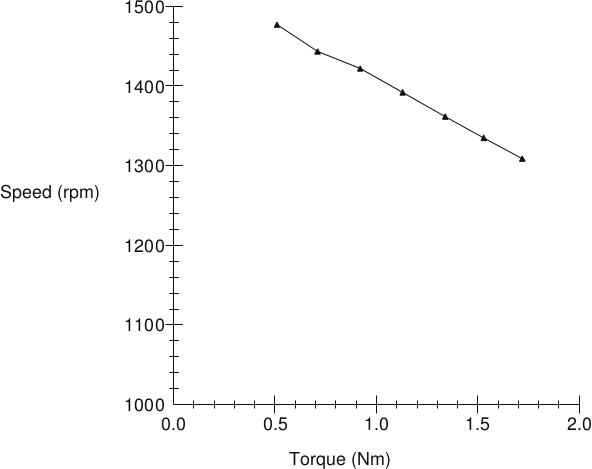
\includegraphics[width=\textwidth]{img/plot4}
    \caption{\textbf{Speed vs. Torque}}
    \label{fig:plot4}
  \end{subfigure}~% The tilde is to keep them side-by-side
%
  \begin{subfigure}[b]{0.45\textwidth}
    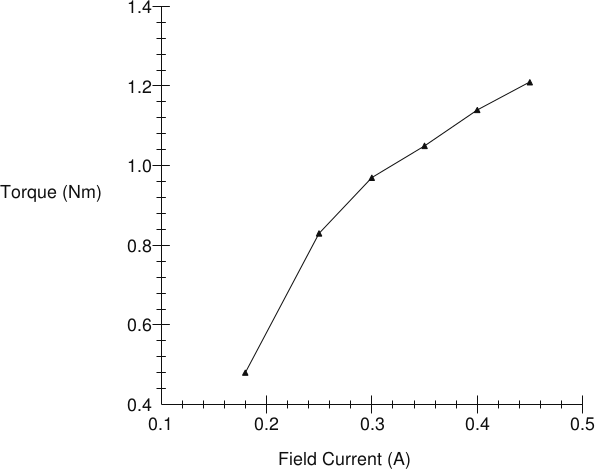
\includegraphics[width=\textwidth]{img/plot5}
    \caption{\textbf{Torque vs. Field Current}}
    \label{fig:plot5}
  \end{subfigure}
\end{figure}

\section*{Conclusions}

%In Figure~\ref{fig:plot_02}, as the \gls{pm} was first starting to increase
%there was a large increase in torque in the opposite direction of motion.
%However, as the \gls{pm} gained rotational speed, the opposition torque

\end{document}
